\documentclass[12pt, a4paper]{article}
\usepackage{caption}
\usepackage{graphicx}
\usepackage{hyperref}
\hypersetup{
    colorlinks,
    citecolor=black,
    filecolor=black,
    linkcolor=black,
    urlcolor=black
}
\usepackage{tikz-network}
\usepackage{amsmath, amsfonts, amssymb, amsthm}
\usepackage{algpseudocode}
\usepackage{algorithm}
\title{Network and Cybersecurity\\ Exercises}
\date{2022}
\author{Kristoffer Klokker}

\usepackage{xcolor,listings}
\usepackage{textcomp}
\usepackage{color}
\usepackage{listings}
\definecolor{codegreen}{rgb}{0,0.6,0}
\definecolor{codegray}{rgb}{0.5,0.5,0.5}
\definecolor{codepurple}{HTML}{C42043}
\definecolor{backcolour}{HTML}{F2F2F2}
\definecolor{bookColor}{cmyk}{0,0,0,0.90}  
\color{bookColor}

\lstset{upquote=true}

\lstdefinestyle{mystyle}{
    backgroundcolor=\color{backcolour},   
    commentstyle=\color{codegreen},
    keywordstyle=\color{codepurple},
    numberstyle=\numberstyle,
    stringstyle=\color{codepurple},
    basicstyle=\footnotesize\ttfamily,
    breakatwhitespace=false,
    breaklines=true,
    captionpos=b,
    keepspaces=true,
    numbers=left,
    numbersep=10pt,
    showspaces=false,
    showstringspaces=false,
    showtabs=false,
    tabsize=3,
}
\lstset{style=mystyle}
\usepackage{zref-base}

\makeatletter
\newcounter{mylstlisting}
\newcounter{mylstlines}
\lst@AddToHook{PreSet}{%
  \stepcounter{mylstlisting}%
  \ifnum\mylstlines=1\relax
    \lstset{numbers=none}
  \else
    \lstset{numbers=left}
  \fi
  \setcounter{mylstlines}{0}%
}
\lst@AddToHook{EveryPar}{%
  \stepcounter{mylstlines}%
}
\lst@AddToHook{ExitVars}{%
  \begingroup
    \zref@wrapper@immediate{%
      \zref@setcurrent{default}{\the\value{mylstlines}}%
      \zref@labelbyprops{mylstlines\the\value{mylstlisting}}{default}%
    }%
  \endgroup
}

% \mylstlines print number of lines inside listing caption
\newcommand*{\mylstlines}{%
  \zref@extractdefault{mylstlines\the\value{mylstlisting}}{default}{0}%
}
\makeatother


\newcommand\numberstyle[1]{%
    \footnotesize
    \color{codegray}%
    \ttfamily
    \ifnum#1<10 0\fi#1 |%
}


\begin{document}
	\maketitle
	\clearpage
	\tableofcontents
	\clearpage
	\section{Preparaiton}
		\subsection{Generalize a formula for sending P such packets back-to-back over the N link}
			For a single package the sending time will be:
			$$d_{end-to-end}=N\frac{L}{R}$$
			For a number of packages $P$ the formular wil lbe:
			$$d_{end-to-end}=(P+N)\frac{L}{R}$$
		\subsection{Consider the circuit-switched network in this figure}
			\begin{figure}[h!]
				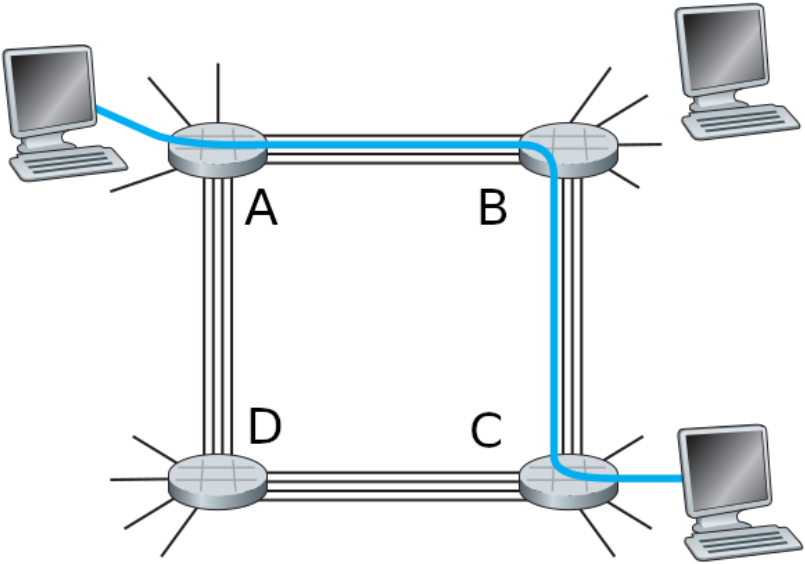
\includegraphics[width=300px]{assets/1.1.png}
				\center
			\end{figure}
			\subsubsection{What is the maximum number of simultaneous conections that can be in progress at the same time in this network}
				Assuming each host can have 4 ingoing and 4 outgoing connections the total number of active connections would be 12. This is where 4 simultaneous connections between the neightboor host.\\
				In case each computer can maximux have 4 ingoing or outgoing connections the total connections would be halfed to 6.
			\subsubsection{Suppose that all connections are between switches A and C. What is the maximum number of simultaneous conections that can be in progress}
				There can only be 4 connections between A and C.
			\subsubsection{Suppose we want to make four connections between switches A and C, and another four connections between B and D. Can we route these calls through the four links to accomodate all eight connections}
				To make a connection one pair can have the two outer links and the other pair can have the two inner links, resulting in 4 links between the pairs.
		\subsection{This elementary problem begins to explore propagation delay and transmission delay, two central concepts in data networking. Consider two hosts, A and B, connected by a single link of rate R bps. Suppose that the two hosts are separated by $m$ meters, and suppose the propagation speed along the link is $s$ meters/sec. Host A is to send a packet of size $L$ bits to Host B}
			\subsubsection{Express the propagation delay, $d_{prop}$ in terms of $m$ and s.}
				
				$$d_{prop} = \frac{m}{s}$$
			\subsubsection{Determine the transmission time of the packet $d_{trans}$ in terms of $L$ and $R$}
				$$d_{trans}=\frac{L}{R}$$
			\subsubsection{ Ignoring processing and queuing delays, obtain an expression for the end-to-end delay}
				$$d_{trans}+d_{prop}=\frac{m}{s}\cdot \frac{L}{R}$$
			\subsubsection{Suppose Host A begins to transmit the packet at time $t=0$. At time $t=d_{trans}$ where is the last of the packet}
				It would be in the link, since it would then have gathered the entire package
			\subsubsection{Suppose $d_{prop}$ is greater than $d_{trans}$. At time $t=d_{trans}$ where si the first bit of the packet.}
				It would be in the link, since the link have to gather the entire package before sending it off
			\subsubsection{Suppose $s=2.5\cdot 10^8$, $L=120$bits and $R=56$kbps. Find the distance $m$ so that $d_{prop}=d_{trans}$}
				\begin{align*}
					d_{trans}=\frac{L}{R}=\frac{120}{56000}=0.00214\\
					d_{prop}=\frac{m}{s}=\frac{m}{2.5\cdot 10^8}=d_{trans}\\
					m=d_{trans}\cdot 2.5\cdot 10^8=535.714
				\end{align*}
				Assuming that $s$ is in the unit meters/sec the distance would be 535.714 meters
		\subsection{Suppose N packets arrive simultaneously to a link at which no packets are currently being transmitted or queued. Each packet is of length L and the link has transmission rate R.}
			\subsubsection{What is the average queing delay for the $n$ packets}
				$$\frac{L\cdot P/2}{R}$$
				On average the packet would be in the middle of queue and therefore be half of $P$
			\subsubsection{Now suppose that N such packets arrive to the link every LN/R seconds. What is the average queuing delay of a packet?}
				Since the package arrival is faster than the package handling time, in the case of an infinite size buffer the aver delay would be infinite
		\subsection{Suppose two hosts A and B are speareated by 20,000 kilometers and are conencted by a direct link of R=2 Mbs. Suppose the propagation speed of the link is $s=2.5\cdot 10^8$ meters/sec}
			\subsubsection{Calculate the bandwidth-delay product $R\cdot d_{prop}$}
				$$R\cdot \frac{m}{s}=2\cdot 10^6b/s\cdot \frac{20,000,000m}{2.5\cdot 10^8m/s}=160Kb$$
			\subsubsection{Consider sending a file of 800,000 bits from Host A to Host B. Suppose the file is sent continuously as one large message. What is the maximum number of bits that will be in the link at any given time}
				160Kb as found in last exercise
			\subsubsection{Provide an interpretation of the bandwidth-delay product}
				Bandwidth-delay product is the number if bits which can exist in the link at one time every second.
			\subsubsection{What is the width of a bit in the link}
				$$\frac{20,000,000m}{160,000b}=125m$$
			\subsubsection{Derive a general expression for the width of a bit in terms of the prpagation speed $s$, the transmission rate $R$ and the length of the link $m$.}
				$$\frac{m}{R\cdot \frac{m}{s}}=\frac{s}{R}$$
		\subsection{Suppose there is a 10 Mbps microwave link between a geostationary satellite and its base station on Earth. Every minut the satellite takes a digital photo and sends it to the base station. Assume a propagation speed of $s=2.5\cdot 10^8$ meters/sec.}
			\subsubsection{What is the propagation delay of the link}
				$$\frac{m}{s}= \frac{35,786,000m}{2.5\cdot 10^8m/s}= 0.143s$$
			\subsubsection{What is the bandwidth delay product of the link}
				$$R\cdot \frac{m}{s}=10^7b\cdot \frac{35,786,000m}{2.5\cdot 10^8m/s}=1.43Mb$$
			\subsubsection{Let x denote the size of the photo. What is the minimum value of x for the microwave link the be contrinously transmitting}
				There are 86400 seconds in a day, therefore the minumum size of the photo would be:
				$$1.43Mb/s \cdot 86400s = 123.5Gb$$
		\subsection{Would it be faster to ship 300 terabytes over night than transfer with 1 Gbps}
			$$\frac{300,000Gb}{1Gb/s}=300,000s= 83.33 hours$$
			it would therefore be faster to ship the harddrive
			
\end{document}
